
%\newpage
\section{Функция самопроверки}
\label{sec:selftest}
Начиная с Версии 0.9k,  реализована функция самопроверки. Использовать ее очень просто. Нужно установить 
испытательный терминал с зажимами, закоротить все зажимы и нажать кнопку \textbf{ TEST}. Программа определяет закороченные 
испытательные зажимы и начинает функцию самопроверки, если Вы подтвердите этот режим повторным нажатием на кнопку 
\textbf{ TEST} в течение 2-х секунд. Это подтверждение необходимо для исключения перехода Тестера в режим самопроверки при 
подключении дефектного транзистора. После окончания самопроверки Тестер начнет обычное измерение. Если никакой 
элемент не будет подключен, то программа закончит работу с выводом сообщения \inquotes{No, unknown, or damaged part}. Вы 
можете запустить самопроверку только на ATmega168 или ATmega328. Перед тестом определяются нулевые сопротивления 
для всех трех комбинаций соединений (T1:T3, T2:T3 и T1:T2). Эти нулевые сопротивления будут учтены при будущих 
измерениях ESR и сопротивлений ниже \(10~\Omega\).
Допустимы только значения нулевого сопротивления ниже \(0.90~\Omega\), поскольку значения этой коррекции
не используется для измерения резисторов выше \(10~\Omega\).
Если Вы используете кабели для измерений, Вы должны использовать только кабели с очень низкими сопротивлением.
Если более поздние результаты измерений сопротивления упадут ниже определенного ранее нулевого значения более, 
чем на \(0,2~\Omega\),
Тестер восстановит режим \inquotes{uncalibrated} (\inquotes{неоткалиброванный}). Во время дальнейших испытаний это будет отмечено 
символом \inquotes{{\_}} (подчеркивание) в конце строки или результата измерений. Каждый шаг функции самопроверки 1 - 7 отображаются в первой 
строке LCD-дисплея символом \inquotes{T}, сопровождаемым номером шага. Каждый шаг повторяется 4 раза, прежде чем программа 
переходит на следующий шаг. Но если Вы держите кнопку \textbf{ TEST} нажатой, когда испытательный цикл закончен, этот тест 
больше не повторяется. Если Вы удерживаете кнопку \textbf{ TEST} нажатой  постоянно, то каждый тест выполняется только 
один раз. 

Без опции AUTO\_CAL в каждом шаге отображаются только результаты измерения, анализ ошибок не выполняется, результаты 
измерений Вы должны интерпретировать сами. В этом месте я дам Вам дополнительный важный совет. Никогда не делайте 
измерения с подключенным разъёмом ISP! Интерфейс ISP искажает измерения.
 
\vspace{1cm}
Вот список осуществляемых в настоящее время тестов:
\vspace{0.5cm}
\begin{enumerate}
\item \textbf{ Измерение \(1,3~V\) (или \(1,1~V\)) опорного напряжения (диапазон изменения опоры).}
В строке 1 текст \inquotes{REF = } и измеренное напряжение, отображенное в \(mV\). Для ATmega8 напряжение должно быть близко 
к \(1,3~V\). Для других микроконтроллеров напряжение должно быть близко к \(1,1~V\). Вторая строка отображает 
результирующий коэффициент для измерения ёмкости с резистором \(470~k\Omega\).
\item \textbf{ Сравнение резисторов \(680~\Omega\).}
В первой строке отображается зашифрованный текст \inquotes{+RL- 12 13 23}. Значение этого текста следующее: RL - обозначение 
низкоомного резистора \(680~\Omega\).

12 - резистор, соединенный с выводом 1 подключен к VCC (\(+5~V\)), а резистор, соединенный с выводом~2 к GND.  
Результат этого измерения отображается во второй строке на первом месте, в виде разницы с теоретическим значением.

13 - резистор, соединенный с выводом 1 подключен к VCC (\(+5~V\)), а резистор, соединенный с выводом~3 к GND.  
Результат этого измерения отображается во второй строке на первом месте, в виде разницы с теоретическим значением.

23 - резистор, соединенный с выводом 2 подключен к VCC (\(+5~V\)), а резистор, соединенный с выводом~3 к GND.  
Результат этого измерения отображается во второй строке на первом месте, в виде разницы с теоретическим значением.

Пожалуйста, помните, что разрешение АЦП составляет приблизительно \(4,88~mV\)! Схемы измерений представлены 
на рисунке~\ref{fig:test2}.
Теоретическое значение с учетом внутреннего сопротивления порта должны быть:
\(\frac{5001 \cdot  (19+680)}{ (19+680+680+22)} = 2493\) .

\begin{figure}[H]
\centering
\begin{overpic}[width=1.\textwidth]{../FIG/Test2.pdf}
  \color{black}
  \put(18,22){\makebox(0,0)[cb]{первое измерение}}
  \put(49,22){\makebox(0,0)[cb]{второе измерение}}
  \put(85,22){\makebox(0,0)[cb]{третье измерение}}
 \end{overpic}
\caption{Сравнение резисторов \(680~\Omega\)}
\label{fig:test2}
\end{figure}

\item \textbf{ Сравнение резисторов \(470~k\Omega\).}
Теперь в первой строке отображается \inquotes{+RH- 12 13 23}. Та же самые действия, как сделано в тесте 2, повторены с 
резисторами \(470~k\Omega\) 
(символы RH).
Все результаты отображают разницу с теоретическим значением. Теоретическое значение с учетом внутреннего 
сопротивления порта вычисляется по формуле:

\(\frac{5001 \cdot (19 + 470000)}{ (19 + 470000 + 470000 + 22)} = 2500\) для всех комбинаций.

\item \textbf{ Отображается сообщение \inquotes{Isolate Probe!}.}
В этом шаге ничего не измеряется. Это означает, что нужно отсоединить \inquotes{закоротку}. 
Этот шаг завершится, как только Вы \inquotes{раcкоротите} входы.

\item \textbf{ Этот тест проверяет способность подключения резисторов \(470~k\Omega\) (RH-) к  GND при подтягивании 
испытательных контактов к GND.}
Первая строка показывает текст \inquotes{RH-}.
Вторая строка должна  показать ноль для всех трех выводов.

\item \textbf{ Этот тест проверяет способность подключения резисторов \(470~k\Omega\) (RH+) к VCC (\(+5~V\)) при 
подтягивании испытательных контактов к VCC (\(+5~V\)).}
Первая строка показывает текст \inquotes{RH+}.
Результаты во второй строке показывают отличие от VCC (\(+5~V\)) и должны быть близким к нулю. 
Большие отличия от значения 0 для теста 5 и теста 6 являются ошибками, такими как проблема изоляции, утечки 
материала или повреждение порта! 

\item \textbf{ Этот шаг проверяет напряжения резистивного делителя \(470~k\Omega~/~680~\Omega\).}
Отличия напряжений  резистивного делителя \(470~k\Omega\) / \(680~\Omega\) от расчетной величины 
отображается  во второй строке LCD-дисплея для всех трех терминалов. Различие больше, чем 
несколько \(mV\), может быть вызвано применением неправильных значений резисторов.
 
\item \textbf{ Измерение внутреннего сопротивления порта подключением выходных контактов к GND.}
Этот и следующие тесты будут проведены, если выбрана опция AUTO\_CAL. Внутреннее сопротивление порта C с выходами, 
подключенными к GND, измеряется по току через подключенные к VCC (\(+5~V\)) резисторы \(680~\Omega\), смотри 
рисунок~\ref{fig:test7}.
Могут быть измерены только три вывода порта АЦП. Внутреннее сопротивление портов B (PB0, PB2 и PB4) не может быть 
измерено без изменения аппаратных средств. Будем считать, что внутреннее сопротивление порта для различных портов 
практически одинаково. Величина сопротивления будет определена в следующем тесте.
\begin{figure}[H]
\centering
 \begin{overpic}[width=.9\textwidth]{../FIG/Test7.pdf}
  \color{black}
  \put(16,34){\makebox(0,0)[cb]{первое измерение}}
  \put(47,35){\makebox(0,0)[cb]{второе измерение}}
  \put(84,35){\makebox(0,0)[cb]{третье измерение}}
 \end{overpic}
\caption{Измерение внутреннего сопротивления порта C подключением выходных контактов к GND}
\label{fig:test7}
\end{figure}

\item \textbf{ Измерение внутреннего сопротивления порта подключением выходных контактов к VCC (\(+5~V\)).}
Необходимый ток задан резисторами \(680~\Omega\) соединёнными с GND. 
Как видно на рисунке~\ref{fig:test8}, 
это те же самые измерения, как и в тесте 8, только с другой стороны. Следующими шагами вычисляется  
сопротивление: \((VCC - (result of test 8) - (result of test 9)) / 680\).
чтобы получить оба значения  резисторов, напряжение (результат теста 8 или 9) делим на этот ток.

Результаты этого теста будут отображены в первой строке текстом \inquotes{RI\_Hi = }, значение  сопротивления (\(\Omega\)) 
относительно VCC,
во второй строке текст \inquotes{RI\_Lo = }

Начиная с версии 1.06k программного обеспечения, значения выходного сопротивления порта определяются в начале 
каждого измерения. Этот тест только показывает значения.

\begin{figure}[H]
\centering
 \begin{overpic}[width=.9\textwidth]{../FIG/Test8.pdf}
  \color{black}
  \put(16,35){\makebox(0,0)[cb]{первое измерение}}
  \put(47,35){\makebox(0,0)[cb]{второе измерение}}
  \put(84,35){\makebox(0,0)[cb]{третье измерение}}
 \end{overpic}
\caption{Измерение внутреннего сопротивления порта подключением выходных контактов к VCC}
\label{fig:test8}
\end{figure}

\item \textbf{ Измерение смещения нуля при измерении конденсаторов.}
В первой строке после \inquotes{C0} отображаются величины смещения нуля при измерении ёмкости конденсаторов в порядке 
комбинаций испытательных выводов 1:3, 2:3 и 1:2. Все три значения отображаются в \(pF\). В этом измерении не 
учитывают предопределенное смещение нуля. Также измеряется смещение нуля для комбинаций выводов в противоположном 
порядке. Результаты измерений записываются в EEprom, если все значения будут меньше, чем \(190~pF\). Это будет 
зафиксировано отображением текста \inquotes{ОК} во второй  строке. Найденное смещение нуля используется для дальнейших 
измерений ёмкости относительно комбинаций выводов. Если результаты измерений ёмкости упадут ниже определенного 
ранее нулевого значения более, чем на \(20~pF\), Тестер восстановит режим \inquotes{uncalibrated} (\inquotes{неоткалиброванный}). 
Во время дальнейших испытаний это будет отмечено символом \inquotes{\_} (подчеркивание) в конце строки или результата измерений. Имейте в 
виду, что при замене испытательных щупов может потребоваться новое регулирование смещения нуля. Если Вы 
используете провода с зажимами, смещение нуля может быть на \(3~pF\) больше, по сравнению с пустым гнездом.
Если тестер настроен с функцией SamplingADC, то значения нулевой ёмкости определяется в двух направлениях для
всех комбинаций контактов. Причина в том, что нулевая ёмкость измеряется для заряда и разряда всех комбинаций
тестовых контактов отдельно.

\item \textbf{ Подключение конденсатора для измерения низких значений индуктивности}
Если тестер настроен на использование функции SamplingADC, требуется подключение конденсатора известной ёмкости
для вычисления значения индуктивности по измерению резонансной частоты LC-контура при параллельном подключении
во время теста индуктивности катушки.
Практические значения ёмкости должны быть в диапазоне от \(10~nF\) до \(27~nF\).
Подходящий конденсатор должен быть подключен к тестовым выводам TP~1 и TP~3, когда в первой строке отображается
сообщение \inquotes{\mbox{\begin{large}1 \electricC 3~10-30nF(L)\end{large}}}.
Этот же конденсатор должен использоваться позже в качестве параллельно подключаемого к катушке при тесте малых 
индуктивностей по резонансной частоте LC-контура.
Если функция SamplingADC не включена, то этот шаг отсутствует.

\item \textbf{ Подключение конденсатора к испытательным выводам~1 и~3.}
В первой строке LCD-дисплея выводится сообщение \inquotes{\mbox{\begin{large}1 \electricC 3~\textgreater 100nF\end{large}}}. Чтобы подготовиться 
к измерению напряжения смещения компаратора, Вы должны подключить \textbf{ высококачественный} 
конденсатор ёмкостью в диапазоне от  \(100~nF\) до \(20~\mu F\).
Допустимо использование \textbf{ только пленочных} конденсаторов.

\item \textbf{ Измерение смещение компаратора для настройки измерения ёмкости.}
Для получения смещения аналогового компаратора, конденсатор уже должен быть подключен к испытательным выводам 
1 и 3. Конденсатор необходим для поддержания напряжения заряда конденсатора на время измерения разницы между 
напряжением заряда и внутренним опорным напряжением (зона). Если измерение прошло успешно, и величина коррекции 
мала, то в первой строке LCD-дисплея отобразится текст \inquotes{REF C = } и величина коррекции будет записана в  EEprom. 
Используя опцию REF\_C\_KORR, Вы можете добавить дополнительное смещение к автоматически измеренному значению. 
Если Вы выбрали опцию AUTOSCALE\_ADC, масштаб АЦП, полученный после однократного измерения напряжение при 
соединении с VCC и однократного измерения напряжения внутреннего ИОН, будет скорректирован путем сравнения 
напряжения на конденсаторе ниже \(1~V\). Результат измерения отображается во второй строке текстом \inquotes{REF R = }. 
Ваше значение опции REF\_R\_KORR является дополнительным смещением к этому автоматически определенному разностному 
значению.

\end{enumerate}

По окончании тестов в первой строке отображается текст \inquotes{Test End} а во второй строке номер версии программного 
обеспечения. 
Если в Makefile установлена опция  FREQUENCY\_50Hz, то на испытательном выводе 2 генерируется прямоугольный 
сигнал \(50~Hz\) и тот же самый сигнал в противофазе - на испытательном выводе 3. Испытательный вывод 1 
подключается к GND. Ток ограничен резисторами \(680~\Omega\).
Это будет отображено, как  \inquotes{50Hz}, в конце первой строки  LCD-дисплея. Сигнал \(50~Hz\) будет сгенерирован 30 раз 
в течение 2 секунд. Если у Вас есть частотомер или осциллограф, то Вы можете проверить требуемые временные 
характеристики сигнала.
Рисунок~\ref{fig:Frequency50} показывает осциллограмму кривой \(50~Hz\) на обоих испытательных выводах для ATmega 
с кварцем.

\begin{figure}[H]
\centering
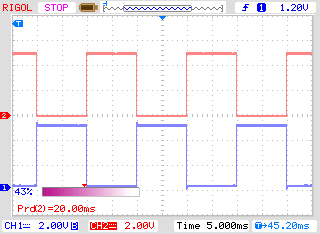
\includegraphics[width=.8\textwidth]{../PNG/Frequency50.png}
\caption{Осциллограмма \(50~Hz\) на выводах 2 и 3}
\label{fig:Frequency50}
\end{figure}

Если Вы не используете кварц, результат может быть неточным. Точная частота и период важны для измерения величины 
ёмкости. Вы можете прервать долговременную генерацию сигнала \(50~Hz\), нажав на кнопку \textbf{ TEST}. Тогда программа 
продолжит обычную задачу измерения.

\subsection{Некоторые результаты функции самопроверки}

На нижеследующих рисунках показаны результаты самопроверок 9 различных микроконтроллеров ATmega168 и 6 
микроконтроллеров ATmega328.

\begin{table}[H]
  \begin{center}
    \begin{tabular}{| l | c | c | c |}
    \hline
Номер теста & Тип измерения & теоретич. зн. & Рисунок \\
    \hline
    \hline
Test 1 & band gap Ref  & 1100 & \ref{fig:SelfTref} \\
    \hline
Test 2 & RL-Mean & 0 & \ref{fig:SelfTMitL} \\
    \hline
Test 3 & RH-Mean & 0 & \ref{fig:SelfTMitH} \\
    \hline
Test 5 & RH-Low &  0 & \ref{fig:SelfTlowH} \\
    \hline
Test 6 & RH-High & 0 & \ref{fig:SelfTtopH} \\
    \hline
Test 8 & R out Lo & 131 & \ref{fig:SelfTRoL} \\
    \hline
Test 9 & R out Hi & 151 & \ref{fig:SelfTRoH} \\
    \hline
Test 10 & Cap zero offset & 30 & \ref{fig:SelfTcap} \\
    \hline
Test 11 & Reference correction & 0 & \ref{fig:SelfTrefKorr} \\
    \hline
    \end{tabular}
  \end{center}
  \caption{Таблица самопроверок}
  \label{tab:test_m168} 
\end{table}

\begin{figure}[H]
\centering
\includegraphics[width=.9\textwidth]{../GNU/SelfTrefRU.pdf}
\caption{Самопроверка: Внутренний ИОН}
\label{fig:SelfTref}
\end{figure}


\begin{figure}[H]
  \begin{subfigure}[b]{.5\textwidth}
    \centering
    \includegraphics[width=1.\textwidth]{../GNU/SelfTMitLRU.pdf}
    \caption{Сопротивление \(680~\Omega\)}
    \label{fig:SelfTMitL}
  \end{subfigure}
  ~
  \begin{subfigure}[b]{.5\textwidth}
    \centering
    \includegraphics[width=1.\textwidth]{../GNU/SelfTMitHRU.pdf}
    \caption{Сопротивление \(470~k\Omega\)}
    \label{fig:SelfTMitH}
  \end{subfigure}
  \caption{Самопроверка: Отклонение среднего напряжения от идеального}
\end{figure}

\begin{figure}[H]
  \begin{subfigure}[b]{.5\textwidth}
  \centering
    \includegraphics[width=1.\textwidth]{../GNU/SelfTbottomHRU.pdf}
    \caption{Сопротивления \(470~k\Omega\) к \(0~V\)}
    \label{fig:SelfTlowH}
  \end{subfigure}
  ~
  \begin{subfigure}[b]{.5\textwidth}
  \centering
    \includegraphics[width=1.\textwidth]{../GNU/SelfTtopHRU.pdf}
    \caption{Сопротивление \(470~k\Omega\) к \(5~V\)}
    \label{fig:SelfTtopH}
  \end{subfigure}
  \caption{Самопроверка: Входное напряжение}
\end{figure}

\begin{figure}[H]
  \begin{subfigure}[b]{.5\textwidth}
  \centering
    \includegraphics[width=1.\textwidth]{../GNU/SelfTRiLoRU.pdf}
    \caption{Сопротивление \(680~\Omega\) к \(5~V\)}
    \label{fig:SelfTRoL}
  \end{subfigure}
  ~
  \begin{subfigure}[b]{.5\textwidth}
  \centering
    \includegraphics[width=1.\textwidth]{../GNU/SelfTRiHiRU.pdf}
    \caption{Сопротивление \(680~\Omega\) к \(0~V\)}
    \label{fig:SelfTRoH}
  \end{subfigure}
  \caption{Самопроверка: Выходное сопротивление}
\end{figure}

\begin{figure}[H]
  \centering
  \includegraphics[width=.9\textwidth]{../GNU/SelfTcap0RU.pdf}
  \caption{Самопроверка: Смещение нуля при измерении ёмкости}
  \label{fig:SelfTcap}
\end{figure}

\begin{figure}[H]
  \centering
  \includegraphics[width=.9\textwidth]{../GNU/SelfTrefKorrRU.pdf}
  \caption{Самопроверка: Величина коррекции после автокалибровки}
  \label{fig:SelfTrefKorr}
\end{figure}

Наконец, я хотел бы показать Вам на рисунке~\ref{fig:SelfTrefDiff}  различие внешнего напряжения на выводе AREF, 
измеренного мультиметром, и измеренного внутренним  АЦП опорного напряжения для 15 различных ATmega и найденных 
напряжений коррекции (REF\_R\_KORR) после автокалибровки рисунок~\ref{fig:SelfTrefDiff}.
Вы можете видеть, что значения автокалибровки почти соответствуют внешним измеренным значениям.

\begin{figure}[H]
  \centering
  \includegraphics[width=.9\textwidth]{../GNU/SelfTrefDiffRU.pdf}
  \caption{Самопроверка: Различие напряжений ИОН, замеренных на внешнем выводе мультиметром и внутренним АЦП}
  \label{fig:SelfTrefDiff}
\end{figure}

